\begin{figure}[t]
\captionsetup[subfigure]{justification=centering}
\centering
%
\begin{subfigure}{.47\textwidth}
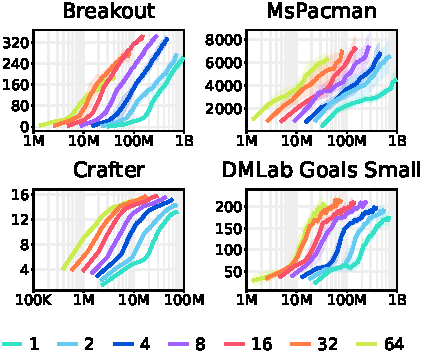
\includegraphics[width=\linewidth]{scaling/scaling_train}
\caption{Training Ratio}
\end{subfigure}%
\hfill%
\begin{subfigure}{.47\textwidth}
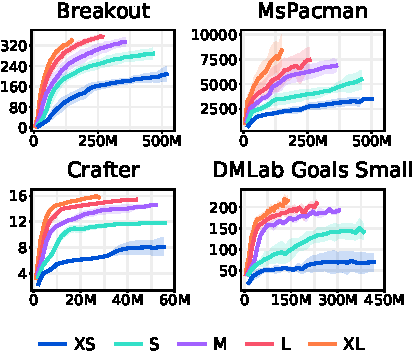
\includegraphics[width=\linewidth]{scaling/scaling_model}
\caption{Model Size}
\end{subfigure}%
\vspace{-1ex}%
\caption{Scaling properties of DreamerV3. The graphs show task performance over environment steps for different training ratios and model sizes reaching from 8M to 200M parameters. The training ratio is the ratio of replayed steps to environment steps. The model sizes are detailed in \cref{tab:models}. Higher training ratios result in substantially improved data-efficiency. Notably, larger models achieve not only higher final performance but also higher data-efficiency.}
\label{fig:scaling}
\end{figure}
